% Options for packages loaded elsewhere
\PassOptionsToPackage{unicode}{hyperref}
\PassOptionsToPackage{hyphens}{url}
\PassOptionsToPackage{dvipsnames,svgnames,x11names}{xcolor}
%
\documentclass[
]{article}

\usepackage{amsmath,amssymb}
\usepackage{iftex}
\ifPDFTeX
  \usepackage[T1]{fontenc}
  \usepackage[utf8]{inputenc}
  \usepackage{textcomp} % provide euro and other symbols
\else % if luatex or xetex
  \usepackage{unicode-math}
  \defaultfontfeatures{Scale=MatchLowercase}
  \defaultfontfeatures[\rmfamily]{Ligatures=TeX,Scale=1}
\fi
\usepackage{lmodern}
\ifPDFTeX\else  
    % xetex/luatex font selection
  \setmainfont[]{Latin Modern Roman}
  \setmathfont[]{Latin Modern Math}
\fi
% Use upquote if available, for straight quotes in verbatim environments
\IfFileExists{upquote.sty}{\usepackage{upquote}}{}
\IfFileExists{microtype.sty}{% use microtype if available
  \usepackage[]{microtype}
  \UseMicrotypeSet[protrusion]{basicmath} % disable protrusion for tt fonts
}{}
\makeatletter
\@ifundefined{KOMAClassName}{% if non-KOMA class
  \IfFileExists{parskip.sty}{%
    \usepackage{parskip}
  }{% else
    \setlength{\parindent}{0pt}
    \setlength{\parskip}{6pt plus 2pt minus 1pt}}
}{% if KOMA class
  \KOMAoptions{parskip=half}}
\makeatother
\usepackage{xcolor}
\setlength{\emergencystretch}{3em} % prevent overfull lines
\setcounter{secnumdepth}{5}
% Make \paragraph and \subparagraph free-standing
\ifx\paragraph\undefined\else
  \let\oldparagraph\paragraph
  \renewcommand{\paragraph}[1]{\oldparagraph{#1}\mbox{}}
\fi
\ifx\subparagraph\undefined\else
  \let\oldsubparagraph\subparagraph
  \renewcommand{\subparagraph}[1]{\oldsubparagraph{#1}\mbox{}}
\fi


\providecommand{\tightlist}{%
  \setlength{\itemsep}{0pt}\setlength{\parskip}{0pt}}\usepackage{longtable,booktabs,array}
\usepackage{calc} % for calculating minipage widths
% Correct order of tables after \paragraph or \subparagraph
\usepackage{etoolbox}
\makeatletter
\patchcmd\longtable{\par}{\if@noskipsec\mbox{}\fi\par}{}{}
\makeatother
% Allow footnotes in longtable head/foot
\IfFileExists{footnotehyper.sty}{\usepackage{footnotehyper}}{\usepackage{footnote}}
\makesavenoteenv{longtable}
\usepackage{graphicx}
\makeatletter
\def\maxwidth{\ifdim\Gin@nat@width>\linewidth\linewidth\else\Gin@nat@width\fi}
\def\maxheight{\ifdim\Gin@nat@height>\textheight\textheight\else\Gin@nat@height\fi}
\makeatother
% Scale images if necessary, so that they will not overflow the page
% margins by default, and it is still possible to overwrite the defaults
% using explicit options in \includegraphics[width, height, ...]{}
\setkeys{Gin}{width=\maxwidth,height=\maxheight,keepaspectratio}
% Set default figure placement to htbp
\makeatletter
\def\fps@figure{htbp}
\makeatother

\usepackage{arxiv}
\usepackage{orcidlink}
\usepackage{amsmath}
\usepackage[T1]{fontenc}
\makeatletter
\@ifpackageloaded{caption}{}{\usepackage{caption}}
\AtBeginDocument{%
\ifdefined\contentsname
  \renewcommand*\contentsname{Table of contents}
\else
  \newcommand\contentsname{Table of contents}
\fi
\ifdefined\listfigurename
  \renewcommand*\listfigurename{List of Figures}
\else
  \newcommand\listfigurename{List of Figures}
\fi
\ifdefined\listtablename
  \renewcommand*\listtablename{List of Tables}
\else
  \newcommand\listtablename{List of Tables}
\fi
\ifdefined\figurename
  \renewcommand*\figurename{Figure}
\else
  \newcommand\figurename{Figure}
\fi
\ifdefined\tablename
  \renewcommand*\tablename{Table}
\else
  \newcommand\tablename{Table}
\fi
}
\@ifpackageloaded{float}{}{\usepackage{float}}
\floatstyle{ruled}
\@ifundefined{c@chapter}{\newfloat{codelisting}{h}{lop}}{\newfloat{codelisting}{h}{lop}[chapter]}
\floatname{codelisting}{Listing}
\newcommand*\listoflistings{\listof{codelisting}{List of Listings}}
\makeatother
\makeatletter
\makeatother
\makeatletter
\@ifpackageloaded{caption}{}{\usepackage{caption}}
\@ifpackageloaded{subcaption}{}{\usepackage{subcaption}}
\makeatother
\ifLuaTeX
  \usepackage{selnolig}  % disable illegal ligatures
\fi
\usepackage{bookmark}

\IfFileExists{xurl.sty}{\usepackage{xurl}}{} % add URL line breaks if available
\urlstyle{same} % disable monospaced font for URLs
\hypersetup{
  pdftitle={The Unexpected Direct Relationship of Walkability on Diabetes Prevalence in the Southern United States},
  pdfauthor={Arkaprabho Bose; Sebastian Oberg; Abhinav Cheruvu},
  colorlinks=true,
  linkcolor={blue},
  filecolor={Maroon},
  citecolor={Blue},
  urlcolor={Blue},
  pdfcreator={LaTeX via pandoc}}

\newcommand{\runninghead}{A Preprint }
\renewcommand{\runninghead}{A Preprint }
\title{The Unexpected Direct Relationship of Walkability on Diabetes
Prevalence in the Southern United States}
\def\asep{\\\\\\ } % default: all authors on same column
\author{\textbf{Arkaprabho
Bose}~\orcidlink{0000-0003-2402-304X}\\Undergraduate Program in
Department of Computer Science\\Texas A \& M University\\College
Station,
TX,\ 77843\\\href{mailto:abose0267@tamu.edu}{abose0267@tamu.edu}\asep\textbf{Sebastian
Oberg}\\Undergraduate Program in Department of Computer Science\\Texas A
\& M University\\College Station, TX,\ 77843\\\asep\textbf{Abhinav
Cheruvu}\\Undergraduate Program in Department of Mathematics\\Texas A \&
M University\\College Station, TX,\ 77843\\}
\date{}
\begin{document}
\maketitle
\begin{abstract}
The diabetes epidemic in the United States, influenced by factors such
as socioeconomic status and climate, presents a nuanced public health
challenge. While the impact of these factors is well-documented, the
influence of walkability on diabetes prevalence has been less explored.
This study investigates how both socioeconomic and climate variables,
alongside walkability, affect diabetes prevalence in the Southern U.S.
Contrary to expectations, our findings indicate that higher walkability
indexes correlate with an increase in diabetes prevalence. This anomaly
persists even when controlling for high blood pressure and low physical
activity, which indicates significant regional variance. Our findings
show that the relationship between walkability and diabetes prevalence
varies significantly by region, driven by distinct socioeconomic and
environmental contexts. This variability highlights the need for public
health strategies and urban planning that are tailored to the specific
regional characteristics to effectively address diabetes.
\end{abstract}

\section{Introduction}\label{sec-intro}

\subsection{Central Thesis Support}\label{central-thesis-support}

What is so important about diabetes?

Does a high walkability index always lead to a lower diabetes
prevalence?

In southern regions, a higher walkability index contributes to diabetes
prevalence

This is significant because it will show where diabetes needs more
preventative measures

\subsection{Paragraph}\label{paragraph}

In this paragraph, we will discuss the importance of the diabetes
epidemic. This could include using statistics from qualified sources to
show how severe it is and how it needs to be addressed. This paragraph
could also discuss the ways that diabetes is currently being combated,
including walkability.

In the second paragraph, we discuss the current believe that a higher
walkability means that there is a lower chance of diabetes prevalence.
we can discuss specific examples where this might not always be the
case.

In the third paragraph, we will discuss our thesis statement. We can
discuss that this is not always the case and that in the eastern US,
walkability actually tends to contribute to diabetes prevalence.

In the 4th paragraph, we can discuss why this finding is important.
Specifically, we will talk about the different ways that this
information can be used to prevent the increase of diabetes prevalence
in the United States.

\section{Related Works}\label{related-works}

\subsection{Central Thesis Support}\label{central-thesis-support-1}

Paragraph 1: Exploring how location affects diabetes risk, focusing on
two studies

Topic: Introduction to how geographical and environmental factors
influence diabetes risk Support: Discuss the relevance of location in
epidemiological studies, which sets the stage for a deeper exploration
of the key studies

Paragraph 2: One study shows that in Northeastern Germany, local factors
like socio-economic status impact diabetes risk

Topic: Detailed analysis of the study conducted in Northeastern Germany
Support: Describe how this research found that socio-economic status
impacts diabetes risk within this specific location Reference the study
to emphasize the importance of local factors in assessing diabetes risk

Paragraph 3: Another study links diabetes with obesity and inactivity,
stressing location-specific health solutions

Topic: Examine another study that correlates diabetes prevalence with
obesity and physical inactivity Support: Highlight findings that stress
the need for location-specific health solutions, highlighting the
importance of understanding local health behaviors and lifestyle factors

Paragraph 4: These insights guide our analysis of walkability's
influence on diabetes in the Southern United States

Topic: Integrate the insights gained from the mentioned studies and
their application to the Southern U.S. context Support: Explain how
these studies guide and inform the analysis of walkability's influence
on diabetes in the Southern U.S., setting up the premise that
walkability might play a similar or different role depending on regional
characteristics

\section{Methods}\label{methods}

\begin{verbatim}
Take a cup of tea and have a break, it will take a few minutes.
          -----A kind suggestion from GWmodel development group
Adaptive bandwidth: 2012 CV score: 26532.61 
Adaptive bandwidth: 1251 CV score: 26549.75 
Adaptive bandwidth: 2482 CV score: 26525.21 
Adaptive bandwidth: 2773 CV score: 26521.91 
Adaptive bandwidth: 2952 CV score: 26520.16 
Adaptive bandwidth: 3064 CV score: 26519.12 
Adaptive bandwidth: 3132 CV score: 26518.4 
Adaptive bandwidth: 3175 CV score: 26517.99 
Adaptive bandwidth: 3201 CV score: 26517.61 
Adaptive bandwidth: 3217 CV score: 26517.29 
Adaptive bandwidth: 3227 CV score: 26517.03 
Adaptive bandwidth: 3233 CV score: 26516.78 
Adaptive bandwidth: 3237 CV score: 26516.61 
Adaptive bandwidth: 3239 CV score: 26516.5 
Adaptive bandwidth: 3241 CV score: 26516.44 
Adaptive bandwidth: 3241 CV score: 26516.44 
\end{verbatim}

\begin{verbatim}
   ***********************************************************************
   *                       Package   GWmodel                             *
   ***********************************************************************
   Program starts at: 2024-04-15 21:35:16.454977 
   Call:
   gwr.basic(formula = DIABETES_CrudePrev ~ NatWalkInd + OBESITY_CrudePrev + 
    BPHIGH_CrudePrev + LPA_CrudePrev + CSMOKING_CrudePrev + AvgSummerTemp + 
    MedianHHIncome, data = data_sp, bw = merged_gwr_bw, kernel = "exponential")

   Dependent (y) variable:  DIABETES_CrudePrev
   Independent variables:  NatWalkInd OBESITY_CrudePrev BPHIGH_CrudePrev LPA_CrudePrev CSMOKING_CrudePrev AvgSummerTemp MedianHHIncome
   Number of data points: 3244
   ***********************************************************************
   *                    Results of Global Regression                     *
   ***********************************************************************

   Call:
    lm(formula = formula, data = data)

   Residuals:
    Min      1Q  Median      3Q     Max 
-5.1987 -2.4505 -0.0327  2.4812  5.3376 

   Coefficients:
                        Estimate Std. Error t value Pr(>|t|)    
   (Intercept)         1.405e+01  8.318e-01  16.892   <2e-16 ***
   NatWalkInd          2.557e-02  5.735e-02   0.446   0.6558    
   OBESITY_CrudePrev   1.366e-03  8.616e-03   0.159   0.8740    
   BPHIGH_CrudePrev   -4.076e-04  8.522e-03  -0.048   0.9619    
   LPA_CrudePrev      -1.263e-02  6.987e-03  -1.808   0.0707 .  
   CSMOKING_CrudePrev  2.104e-02  1.147e-02   1.835   0.0666 .  
   AvgSummerTemp       6.979e-03  5.825e-03   1.198   0.2310    
   MedianHHIncome      3.037e-07  2.473e-06   0.123   0.9022    

   ---Significance stars
   Signif. codes:  0 '***' 0.001 '**' 0.01 '*' 0.05 '.' 0.1 ' ' 1 
   Residual standard error: 2.855 on 3236 degrees of freedom
   Multiple R-squared: 0.00256
   Adjusted R-squared: 0.0004027 
   F-statistic: 1.187 on 7 and 3236 DF,  p-value: 0.3067 
   ***Extra Diagnostic information
   Residual sum of squares: 26372.17
   Sigma(hat): 2.852111
   AIC:  16021.88
   AICc:  16021.94
   BIC:  12905.4
   ***********************************************************************
   *          Results of Geographically Weighted Regression              *
   ***********************************************************************

   *********************Model calibration information*********************
   Kernel function: exponential 
   Fixed bandwidth: 3241 
   Regression points: the same locations as observations are used.
   Distance metric: Euclidean distance metric is used.

   ****************Summary of GWR coefficient estimates:******************
                             Min.     1st Qu.      Median     3rd Qu.    Max.
   Intercept           1.4045e+01  1.4046e+01  1.4047e+01  1.4049e+01 14.0506
   NatWalkInd          2.5473e-02  2.5635e-02  2.5714e-02  2.5756e-02  0.0258
   OBESITY_CrudePrev   1.3241e-03  1.3425e-03  1.3717e-03  1.3898e-03  0.0014
   BPHIGH_CrudePrev   -4.4621e-04 -4.2821e-04 -4.0579e-04 -3.8442e-04 -0.0004
   LPA_CrudePrev      -1.2650e-02 -1.2626e-02 -1.2608e-02 -1.2602e-02 -0.0126
   CSMOKING_CrudePrev  2.0954e-02  2.1004e-02  2.1071e-02  2.1117e-02  0.0211
   AvgSummerTemp       6.9699e-03  6.9812e-03  6.9854e-03  6.9881e-03  0.0070
   MedianHHIncome      2.8750e-07  2.9627e-07  3.0689e-07  3.1591e-07  0.0000
   ************************Diagnostic information*************************
   Number of data points: 3244 
   Effective number of parameters (2trace(S) - trace(S'S)): 8.110786 
   Effective degrees of freedom (n-2trace(S) + trace(S'S)): 3235.889 
   AICc (GWR book, Fotheringham, et al. 2002, p. 61, eq 2.33): 16021.95 
   AIC (GWR book, Fotheringham, et al. 2002,GWR p. 96, eq. 4.22): 16011.84 
   BIC (GWR book, Fotheringham, et al. 2002,GWR p. 61, eq. 2.34): 12824.91 
   Residual sum of squares: 26371.36 
   R-square value:  0.002590885 
   Adjusted R-square value:  9.009731e-05 

   ***********************************************************************
   Program stops at: 2024-04-15 21:35:17.698256 
\end{verbatim}

\subsection{Central Thesis Support}\label{central-thesis-support-2}

In order to analyze diabetes as a response of walkability, we need good,
clean data

In order to make sure that walkability is consistent as a coefficient,
we choose multiple covariates that might be significant

We used GWR to create coefficient surfaces to analyze which parts of the
country had the most impact on diabetes

We compared GWR with Random Forest to show that GWR is not overfitting,
to prevent error

\subsection{Paragraphs}\label{paragraphs}

In the first paragraph, we will talk about the importance of good, clean
data. In addition to this, we will also talk about what data we will be
analyzing, and where we got it

In the second paragraph, we can discuss the reasoning behind choosing
the covariates that we did. This can be a good segue into talking about
the GWR, and how we went about cleaning the data.

In the next paragraph, we can talk about how the model was used, and
tuned to fit our data. Specifically how we chose a bandwidth and what
package we used.

In the last paragraph, we can discuss the plots. In the paragraph, we
discuss the ways the different plots were created (facet plots etc.)

\section{Results}\label{results}

\subsection{Central Thesis Level
Outline}\label{central-thesis-level-outline}

Paragraph 1: Diabetes Prevalence in The South

Topic: There is a clear positive relationship between walkability and
diabetes in the Southern Region. Support: From the plots,the estimated
impact of walkability on diabetes is consistently higher in the southern
to South East region. These areas tend to be red, which is associated
with a higher impact of walkability on diabetes prevalence.

Paragraph 2: Certain reasons why walkability has a positive relationship
with diabetes prevalence in the South.

Topic: Higher temperatures may be a potential reason why Walkability has
a positive relationship with Diabetes in the South. Support: As seen by
the plot, in colder regions such as the west coast and in the Pacific
Northwest, there is negative impact of Walkability on Diabetes. Thus,
this shows that higher temperatures in the South may lead to people
staying indoors, reducing walkability and in turn possibly leading to
higher diabetes rates.

Paragraph 3: Other factors that potentially lead to higher Diabetes
prevalence

Topic: Additional Risk factors beside Walkability on Diabetes Support:
Overall, certain risk factors such as smoking, obesity, etc. had a high
impact on diabetes in every region. We expected this to be the case,
further supporting our thesis.

Paragraph 4: Validation metrics

Topic: Our model's performance overall

Support: From the residual plot, we can see that the points are
scattered fairly evenly around and the residual plot does not have a
specific pattern, indicating a well-fit model. This further supports our
central thesis indiciating that the model we fit is performing well.

From the plots, it shows that the southern region of the United States,
walkability had a postive relationship with diabetes prevalence.

From the GWR model's spatial plot which shows the estimated impact of
the National Walkability Index it is clear that there is a negative
relationship between Walkability and Diabetes.

In the Western Region, though, there is a more positive relationship
between the impact of Walkability and Diabetes in the Southern and
Eastern Region further supporting our central thesis.

\begin{verbatim}
Reading layer `tl_2023_us_county' from data source 
  `/Users/arkaprabhobose/Spatiotemporal_Analysis_of_Diabetes_Incidence/data/shapes/us_counties' 
  using driver `ESRI Shapefile'
Simple feature collection with 3235 features and 18 fields
Geometry type: MULTIPOLYGON
Dimension:     XY
Bounding box:  xmin: -179.2311 ymin: -14.60181 xmax: 179.8597 ymax: 71.43979
Geodetic CRS:  NAD83
\end{verbatim}

\begin{verbatim}
Warning: Returning more (or less) than 1 row per `summarise()` group was deprecated in
dplyr 1.1.0.
i Please use `reframe()` instead.
i When switching from `summarise()` to `reframe()`, remember that `reframe()`
  always returns an ungrouped data frame and adjust accordingly.
\end{verbatim}

\begin{verbatim}
`summarise()` has grouped output by 'CountyFIPS'. You can override using the
`.groups` argument.
\end{verbatim}

\begin{verbatim}
Warning in clean_income(.): NAs introduced by coercion
\end{verbatim}

\begin{verbatim}
  CountyFIPS          NatWalkInd      StateAbbr         DIABETES_CrudePrev
 Length:3079        Min.   : 2.722   Length:3079        Min.   : 5.262    
 Class :character   1st Qu.: 5.267   Class :character   1st Qu.:10.468    
 Mode  :character   Median : 6.076   Mode  :character   Median :11.950    
                    Mean   : 6.473                      Mean   :12.194    
                    3rd Qu.: 7.027                      3rd Qu.:13.857    
                    Max.   :15.957                      Max.   :24.200    
 BPHIGH_CrudePrev OBESITY_CrudePrev LPA_CrudePrev   CSMOKING_CrudePrev
 Min.   :19.57    Min.   :16.21     Min.   :12.80   Min.   : 6.991    
 1st Qu.:33.10    1st Qu.:33.50     1st Qu.:27.36   1st Qu.:17.777    
 Median :36.23    Median :36.33     Median :30.90   Median :20.300    
 Mean   :36.56    Mean   :35.88     Mean   :31.03   Mean   :20.590    
 3rd Qu.:40.27    3rd Qu.:38.53     3rd Qu.:34.90   3rd Qu.:23.276    
 Max.   :56.73    Max.   :52.00     Max.   :51.77   Max.   :39.400    
    avg_temp      Median.Household.Income   INTPTLAT           INTPTLON        
 Min.   : 70.66   Min.   : 24732          Length:3079        Length:3079       
 1st Qu.: 84.68   1st Qu.: 46132          Class :character   Class :character  
 Median : 88.60   Median : 53115          Mode  :character   Mode  :character  
 Mean   : 91.06   Mean   : 55314                                               
 3rd Qu.: 95.48   3rd Qu.: 61520                                               
 Max.   :129.31   Max.   :151806                                               
          geometry   
 MULTIPOLYGON :3079  
 epsg:4269    :   0  
 +proj=long...:   0  
                     
                     
                     
\end{verbatim}

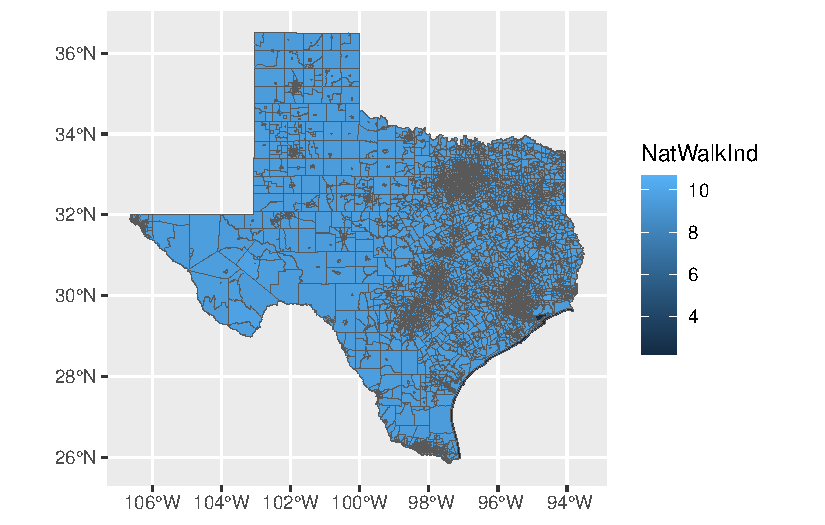
\includegraphics{report_files/figure-pdf/unnamed-chunk-5-1.pdf}

\begin{verbatim}
$corr
                        CSMOKING_CrudePrev DIABETES_CrudePrev BPHIGH_CrudePrev
CSMOKING_CrudePrev               1.0000000         0.65410870        0.6543203
DIABETES_CrudePrev               0.6541087         1.00000000        0.8906639
BPHIGH_CrudePrev                 0.6543203         0.89066387        1.0000000
OBESITY_CrudePrev                0.6908164         0.74185885        0.7341979
LPA_CrudePrev                    0.7575053         0.82350117        0.7900507
avg_temp                        -0.2668859         0.01707046       -0.1501691
NatWalkInd                      -0.5027294        -0.44541593       -0.5474346
Median.Household.Income         -0.6427970        -0.70478574       -0.6648329
                        OBESITY_CrudePrev LPA_CrudePrev    avg_temp NatWalkInd
CSMOKING_CrudePrev              0.6908164     0.7575053 -0.26688592 -0.5027294
DIABETES_CrudePrev              0.7418588     0.8235012  0.01707046 -0.4454159
BPHIGH_CrudePrev                0.7341979     0.7900507 -0.15016908 -0.5474346
OBESITY_CrudePrev               1.0000000     0.7976565 -0.13164311 -0.4776442
LPA_CrudePrev                   0.7976565     1.0000000 -0.03142030 -0.4428780
avg_temp                       -0.1316431    -0.0314203  1.00000000  0.2888152
NatWalkInd                     -0.4776442    -0.4428780  0.28881523  1.0000000
Median.Household.Income        -0.5888337    -0.6961082  0.03689081  0.4429536
                        Median.Household.Income
CSMOKING_CrudePrev                  -0.64279700
DIABETES_CrudePrev                  -0.70478574
BPHIGH_CrudePrev                    -0.66483292
OBESITY_CrudePrev                   -0.58883372
LPA_CrudePrev                       -0.69610817
avg_temp                             0.03689081
NatWalkInd                           0.44295364
Median.Household.Income              1.00000000

$corrPos
                     xName                   yName x y        corr
1       CSMOKING_CrudePrev      CSMOKING_CrudePrev 1 8  1.00000000
2       DIABETES_CrudePrev      CSMOKING_CrudePrev 2 8  0.65410870
3       DIABETES_CrudePrev      DIABETES_CrudePrev 2 7  1.00000000
4         BPHIGH_CrudePrev      CSMOKING_CrudePrev 3 8  0.65432027
5         BPHIGH_CrudePrev      DIABETES_CrudePrev 3 7  0.89066387
6         BPHIGH_CrudePrev        BPHIGH_CrudePrev 3 6  1.00000000
7        OBESITY_CrudePrev      CSMOKING_CrudePrev 4 8  0.69081644
8        OBESITY_CrudePrev      DIABETES_CrudePrev 4 7  0.74185885
9        OBESITY_CrudePrev        BPHIGH_CrudePrev 4 6  0.73419790
10       OBESITY_CrudePrev       OBESITY_CrudePrev 4 5  1.00000000
11           LPA_CrudePrev      CSMOKING_CrudePrev 5 8  0.75750526
12           LPA_CrudePrev      DIABETES_CrudePrev 5 7  0.82350117
13           LPA_CrudePrev        BPHIGH_CrudePrev 5 6  0.79005070
14           LPA_CrudePrev       OBESITY_CrudePrev 5 5  0.79765650
15           LPA_CrudePrev           LPA_CrudePrev 5 4  1.00000000
16                avg_temp      CSMOKING_CrudePrev 6 8 -0.26688592
17                avg_temp      DIABETES_CrudePrev 6 7  0.01707046
18                avg_temp        BPHIGH_CrudePrev 6 6 -0.15016908
19                avg_temp       OBESITY_CrudePrev 6 5 -0.13164311
20                avg_temp           LPA_CrudePrev 6 4 -0.03142030
21                avg_temp                avg_temp 6 3  1.00000000
22              NatWalkInd      CSMOKING_CrudePrev 7 8 -0.50272937
23              NatWalkInd      DIABETES_CrudePrev 7 7 -0.44541593
24              NatWalkInd        BPHIGH_CrudePrev 7 6 -0.54743455
25              NatWalkInd       OBESITY_CrudePrev 7 5 -0.47764419
26              NatWalkInd           LPA_CrudePrev 7 4 -0.44287799
27              NatWalkInd                avg_temp 7 3  0.28881523
28              NatWalkInd              NatWalkInd 7 2  1.00000000
29 Median.Household.Income      CSMOKING_CrudePrev 8 8 -0.64279700
30 Median.Household.Income      DIABETES_CrudePrev 8 7 -0.70478574
31 Median.Household.Income        BPHIGH_CrudePrev 8 6 -0.66483292
32 Median.Household.Income       OBESITY_CrudePrev 8 5 -0.58883372
33 Median.Household.Income           LPA_CrudePrev 8 4 -0.69610817
34 Median.Household.Income                avg_temp 8 3  0.03689081
35 Median.Household.Income              NatWalkInd 8 2  0.44295364
36 Median.Household.Income Median.Household.Income 8 1  1.00000000

$arg
$arg$type
[1] "upper"
\end{verbatim}

\begin{verbatim}
Take a cup of tea and have a break, it will take a few minutes.
          -----A kind suggestion from GWmodel development group
Fixed bandwidth: 35.02304 CV score: 2794.769 
Fixed bandwidth: 21.64976 CV score: 2666.916 
Fixed bandwidth: 13.38461 CV score: 2465.125 
Fixed bandwidth: 8.276475 CV score: 2177.631 
Fixed bandwidth: 5.119471 CV score: 1828.855 
Fixed bandwidth: 3.168336 CV score: 1475.882 
Fixed bandwidth: 1.962468 CV score: 1169.739 
Fixed bandwidth: 1.2172 CV score: 956.5881 
Fixed bandwidth: 0.7565997 CV score: 864.9365 
Fixed bandwidth: 0.4719329 CV score: 898.3396 
Fixed bandwidth: 0.9325335 CV score: 889.8361 
Fixed bandwidth: 0.6478667 CV score: 862.2611 
Fixed bandwidth: 0.580666 CV score: 868.5209 
Fixed bandwidth: 0.689399 CV score: 861.7055 
Fixed bandwidth: 0.7150674 CV score: 862.3952 
Fixed bandwidth: 0.6735351 CV score: 861.6588 
Fixed bandwidth: 0.6637306 CV score: 861.7861 
Fixed bandwidth: 0.6795946 CV score: 861.6406 
Fixed bandwidth: 0.6833395 CV score: 861.6518 
Fixed bandwidth: 0.67728 CV score: 861.6422 
Fixed bandwidth: 0.681025 CV score: 861.6429 
Fixed bandwidth: 0.6787105 CV score: 861.6404 
Fixed bandwidth: 0.6781641 CV score: 861.6408 
Fixed bandwidth: 0.6790482 CV score: 861.6404 
\end{verbatim}

\includegraphics{report_files/figure-pdf/unnamed-chunk-10-1.pdf}

\begin{center}
\includegraphics{impact_plot.png}
\end{center}

\begin{center}
\includegraphics{facet_plot.png}
\end{center}

\section{Discussion}\label{discussion}

\subsection{Central Thesis Support}\label{central-thesis-support-3}

Paragraph 1: Analyzing the relationship between walkability and diabetes
prevalence in our study's context

Topic: Compare and contrast the study's findings on walkability and
diabetes in the Southern U.S. with the existing literature Support:
Analyze how the results align or contrast from the findings in
Northeastern Germany and other relevant studies, which shows the
uniqueness of the Southern U.S. context

Paragraph 2: Comparing our findings with existing research to understand
regional differences

Topic: Mention the regional variations in diabetes prevalence and
walkability discovered during the study Support: Explain how these
variations might be influenced by socioeconomic and environmental
factors specific to different parts of the Southern U.S.

Paragraph 3: Discussing the implications of our study for local health
strategies

Topic: Suggest tailored public health strategies based on our findings
Support: Propose specific interventions and urban planning strategies
that could be effective in regions with varying walkability indices.
Maybe draw parallels to successful approaches in other regions discussed
in the literature

Paragraph 4: Highlighting the need for tailored interventions based on
regional characteristics to combat diabetes

Topic: Reinforce the necessity for region-specific approaches to combat
diabetes effectively Support: Note the broader consequences of the
study's findings for public health policy and urban planning,
emphasizing that one-size-fits-all solutions are not effective in
addressing the nuanced challenges presented by diabetes

\newpage{}

\section*{References}\label{references}
\addcontentsline{toc}{section}{References}



\end{document}
